%!TEX root = ../thesis.tex
%*******************************************************************************
%***************************** Fifth Chapter **********************************
%*******************************************************************************
\graphicspath{{Chapter5/Figs/Vector/}{Chapter5/Figs/}}

%%%%%%%%%%%%%%%%%%%%%%%%%%%%%%%%%%%%%%%%%%%%%%%%%%%%%%%%%%%%%%%%%%%%%%%%%%%%%%%%
% Proposed Portal Solution
%%%%%%%%%%%%%%%%%%%%%%%%%%%%%%%%%%%%%%%%%%%%%%%%%%%%%%%%%%%%%%%%%%%%%%%%%%%%%%%%
% - Is it possible to communicate the inner workings of the system through the
%   user interface?
\chapter{Portal}

% Which backend concepts are essential to display in the frontend?
% Which design practices allow users to understand coherence of different
%  elements that make up a rule?
% How should a user know what the outcome of his interactions with the system
%  are?

%%%%%%%%%%%%%%%%%%%%%%%%%%%%%%%%%%%%%%%%%%%%%%%%%%%%%%%%%%%%%%%%%%%%%%%%%%%%%%%%
% Introduction
%%%%%%%%%%%%%%%%%%%%%%%%%%%%%%%%%%%%%%%%%%%%%%%%%%%%%%%%%%%%%%%%%%%%%%%%%%%%%%%%
% - Which frontend design allows users to reason about complex price rules?
\section{Introduction}
The term 'reasoning' in the title, meaning "the action of thinking about something in a logical, sensible way", may have been redundant if a system were to calculate trip prices autonomously --- this system is designed with the user in mind. That is why the inner workings of the system must be expressed in such a way that given some rule as input, the user will be able to logically derive the consequential output with confidence.

%%%%%%%%%%%%%%%%%%%%%%%%%%%%%%%%%%%%%%%%%%%%%%%%%%%%%%%%%%%%%%%%%%%%%%%%%%%%%%%%
% Visual Hierarchy
%%%%%%%%%%%%%%%%%%%%%%%%%%%%%%%%%%%%%%%%%%%%%%%%%%%%%%%%%%%%%%%%%%%%%%%%%%%%%%%%
%
\section{Design}
A pricing rule is nothing more than a set of prices and collection of criteria by which a trip must abide in order for those prices to apply. These criteria and pricing information are stored in database entities, which could be expressed as components in a view. For example, "the pickup location of a trip must be located in Amsterdam" is a criterion that is stored in a location entity, that may be expressed as polygon on a world map component. Even if the possible combinations of criteria could be graphed, it would be highly dimensional.

\subsection{Essential Components}
The main entities that make up a the price calculation system are visualized in Figure \ref{fig:Treemap}. The plurality of the child entities define whether more than one child are present within the parent entity. For example, rules have many products, with each product having one price, which has one priceFixed and one priceDynamic.

\begin{figure}[H]
	\centering
	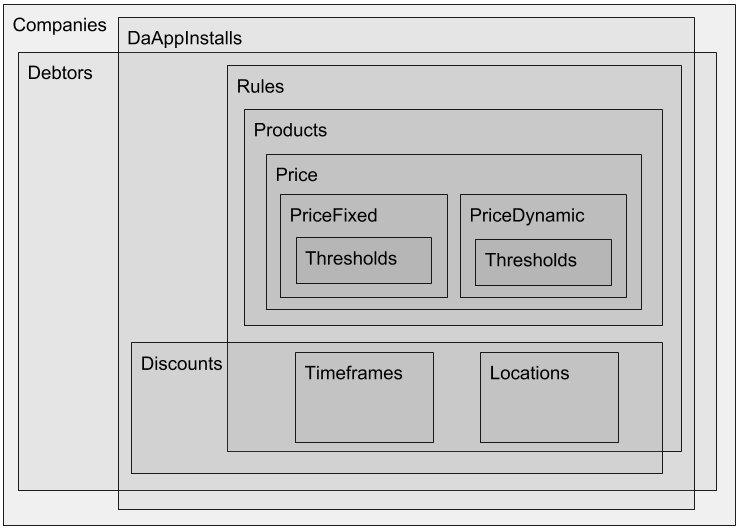
\includegraphics[width=0.7\textwidth]{Treemap}
	\caption[Treemap of Components]{Treemap of components.}
	\label{fig:Treemap}
\end{figure}

\subsection{Expressing Order}
Figure \ref{fig:Treemap} taps into the ability of the reader to preattentively process the images structure. The human brain has already ordered the differently sized boxes by enclosure, proximity, intensity, and spatial grouping. Stephen Few states that "Perception of these basic visual attributes is called 'preattentive' processing, in contrast to the conscious part of perception, which is called 'attentive' processing. Preattentive processing is extremely fast and broadband in that we can simultaneously perceive a large number of these basic visual attributes, called 'preattentive attributes'. Preattentive perception is done in parallel, but attentive processing is done serially and is, therefore, much slower." in \cite[p.~3]{few}. This fact can be used to construct a hierarchy through visual queues. A famous phrase often used in data visualizations called Shneiderman's mantra \cite{mantra}, lays the foundation of principles that enable a user to maintain an understanding of the context in which data is visualized. The sentences in the mantra dictate that there are three stages in data exploration.

\begin{enumerate}
	\item Overview First
	\item Zoom and Filter
	\item Details on Demand
\end{enumerate}

Pricing rules cannot be plotted in a graph, yet this mantra in combination with preattentive attributes could be put to good use in reducing the cognitive overhead while reasoning about pricing rules.

%%%%%%%%%%%%%%%%%%%%%%%%%%%%%%%%%%%%%%%%%%%%%%%%%%%%%%%%%%%%%%%%%%%%%%%%%%%%%%%%
% Design
%%%%%%%%%%%%%%%%%%%%%%%%%%%%%%%%%%%%%%%%%%%%%%%%%%%%%%%%%%%%%%%%%%%%%%%%%%%%%%%%
%
\section{Visual Hierarchy}
In order to communicate the criteria of one pricing rule, the system must guide the user from an overview down to the less important details of the rule. This is to be achieved by splitting up the various criteria into multiple views. What this means is that the user is limited to only reason about a subset of the criteria at once. For example, the user is obligated to first define a location, before it is assigned to a rule, splitting problems into smaller portions. The mantra could be translated into the design on multiple levels.

Entities that are part of a many to many relation, should possibly have their own tabs, overview and detail pages. The reason ...
% reason

Entities with one to one can easily incorporate the relation in the same view ...

Entities with one to many can directly incorporate the components into the same view, if possible (like thresholds) ...


Some components are easy to reason about, and could be combined with other components to make up one view. For example, one rule can have many product entities, and each product has a price entity. These components could compose a single view, having one rule and a list of products with their respective prices. Each view can be categorized as one of the following:

\begin{enumerate}
	\item Overview: enumerates over a list of entities
	\item Detail page: contains one particular entity
	\item Composite page: displays a combination of lists of entities and/or single entities that belong together
\end{enumerate}

The mantra could also be used to present properties of entities in the same fashion. But for each enumeration, a direction of space on the page must be filled. As a webpage only has two dimensions of space, the properties that fill up the space must be grouped in some fashion. Preattentive attributes can be utilized to illustrate that some elements on composite pages belong to eachother, or are in fact distinct.

%%%%%%%%%%%%%%%%%%%%%%%%%%%%%%%%%%%%%%%%%%%%%%%%%%%%%%%%%%%%%%%%%%%%%%%%%%%%%%%%
% Products
%%%%%%%%%%%%%%%%%%%%%%%%%%%%%%%%%%%%%%%%%%%%%%%%%%%%%%%%%%%%%%%%%%%%%%%%%%%%%%%%
%
\section{Products}
Users are allowed to view the list of products that have been created. Products an be selected, upon which the user is taken to the detail page where the type, name and other properties can be set, and where the product may be deleted.

%%%%%%%%%%%%%%%%%%%%%%%%%%%%%%%%%%%%%%%%%%%%%%%%%%%%%%%%%%%%%%%%%%%%%%%%%%%%%%%%
% Timeframes
%%%%%%%%%%%%%%%%%%%%%%%%%%%%%%%%%%%%%%%%%%%%%%%%%%%%%%%%%%%%%%%%%%%%%%%%%%%%%%%%
%
\section{Timeframes}
No overview or detail page has been created for this entity. This is because the reuse potential of this entity is too low, and the belongingness to a rule or discount is too high. Timeframes consist of two dates between which a discount or rule is active.

\subsection{Specific Week Days}
A toggle can be activated so that the hours for each day can be defined.

\begin{figure}[H]
	\centering
	
\includegraphics[width=0.7\textwidth]{Blank}
	\caption[Timeframe Component]{Timeframe with specific week days.}
	\label{fig:Timeframe Component}
\end{figure}

When this toggle is set, the time aspect of the start and end date is hidden.

%%%%%%%%%%%%%%%%%%%%%%%%%%%%%%%%%%%%%%%%%%%%%%%%%%%%%%%%%%%%%%%%%%%%%%%%%%%%%%%%
% Locations
%%%%%%%%%%%%%%%%%%%%%%%%%%%%%%%%%%%%%%%%%%%%%%%%%%%%%%%%%%%%%%%%%%%%%%%%%%%%%%%%
%
\section{Locations}
Locations have been defined as either points or areas. In technical terms, this is sound. For an average user, this does not sound intuative. That is why locations are shown as two groups: locations and areas. In technical terms, and in this chapter, location is used to refer to the entity that can be of type point and area. Again, an overview allows the user to select a location in order to modify or delete it.

\begin{figure}[H]
	\centering
	
\includegraphics[width=0.7\textwidth]{Blank}
	\caption[Locations Overview]{Overview of points and areas.}
	\label{fig:Locations Overview}
\end{figure}

\subsection{Point}
The distinction between points and areas is made in the sense that points are small locations a person could point at, like a house, hotel or a shop. Area's are bigger and more complex locations, like Schiphol or The Hague.

When a point is created, a user searches for a place in Google Places, gives it a name and a descriptor, and saves it as if it were a string of characters that would be matched within the system.

When an existing point is selected, the actual polygon is showing on the map.

\subsection{Area}
The map allows users to have more freedom in describing the location.

When an area is created, the user has the freedom to start drawing on

%%%%%%%%%%%%%%%%%%%%%%%%%%%%%%%%%%%%%%%%%%%%%%%%%%%%%%%%%%%%%%%%%%%%%%%%%%%%%%%%
% Pricing
%%%%%%%%%%%%%%%%%%%%%%%%%%%%%%%%%%%%%%%%%%%%%%%%%%%%%%%%%%%%%%%%%%%%%%%%%%%%%%%%
%
\section{Pricing}
Intro

\subsection{Rules}
Timeframe selector

Location picker

Challenge fitting rule information, prices per products per rule and even thresholds

\subsection{Discounts}
Discounts mirror rule entities

\subsection{Priority}
Sorting by dragging

%%%%%%%%%%%%%%%%%%%%%%%%%%%%%%%%%%%%%%%%%%%%%%%%%%%%%%%%%%%%%%%%%%%%%%%%%%%%%%%%
% Apps
%%%%%%%%%%%%%%%%%%%%%%%%%%%%%%%%%%%%%%%%%%%%%%%%%%%%%%%%%%%%%%%%%%%%%%%%%%%%%%%%
%
\section{Apps}
Apps are included in the overview, while Debtors are not.

Discounts can be enabled for apps

Rules can be linked to apps

Is estimated or fixed can be defined for enabled rules


\section{Premise}
\[\textit{Is it possible to communicate the inner workings of the system through the user interface?}\]\hfill

% Which backend concepts are essential to display in the frontend?
% Which design practices allow users to understand coherence of different elements that make up a rule?
% How should a user know what the outcome of his interactions with the system are?
